%
% Another appendix chapter
\chapter{Towards Application}

% Challenges
\section{Challenges}
\subsection{Angular Momentum and Height Variation}
Normal control framework IHMC:
\begin{equation}
    F_{x} = \frac{x-x_{cmp,d}}{z_0}mg.
\end{equation}
So scaling up $F_x$ with $F_z$ could be an option.
Formulas \ac{CoP} and \ac{CMP}:
\begin{equation}
    x_{cop}=x-\frac{F_x}{F_z}-\frac{\tau_y}{F_z}
\end{equation}
\begin{equation}
    x_{cmp}=x-\frac{F_x}{F_z}
\end{equation}

Special case where \ac{CoM} is above \ac{CoP}:
\begin{align}
     x-x_{cop}=0\\
     \frac{F_x}{F_z}+\frac{\tau_y}{F_z}=0.
\end{align}
Im this situation, scaling up $F_x$ with $F_z$, $\tau_y$ only contributes to $F_x$. So for contribution of added $F_z$, look at \ac{CoP}:
\begin{equation}
    F_{x} = \frac{x-x_{cop}}{z}F_z - \frac{\tau_y}{z}
\end{equation}
The effects of changing the ground reaction compared to the \ac{CMP} and not with the \ac{CoP} are visualized in \figref{fig:cmpFz}
\begin{figure}[h]
  \begin{subfigure}{0.3\textwidth}
  \centering
  \includegraphics[width=.8\linewidth]{STYLESTUFF/2DCMPVIZ.png}
   \caption{}
    \label{fig:cmpFza}
  \end{subfigure}
  \begin{subfigure}{0.3\textwidth}
    \centering
  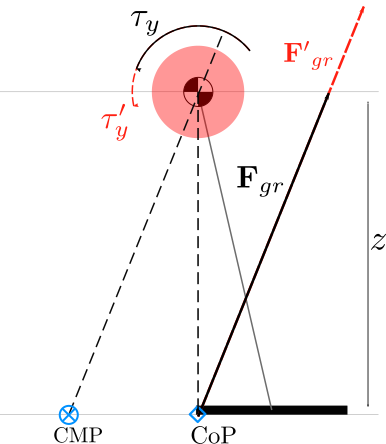
\includegraphics[width=.8\linewidth]{STYLESTUFF/2DCMPVIZCoPzero.png}
  \caption{}
   \label{fig:cmpFzb}
  \end{subfigure}
  \begin{subfigure}{0.36\textwidth}
    \centering
  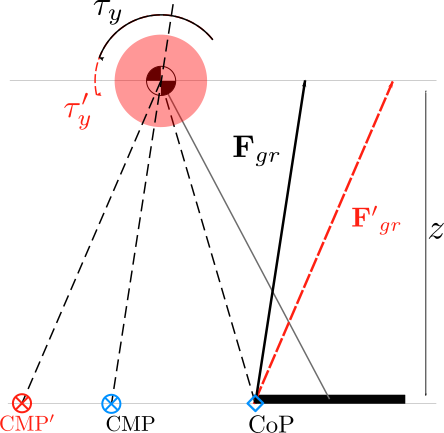
\includegraphics[width=.8\linewidth]{STYLESTUFF/2DCMPVIZFgradjusted.png}
    \caption{}
     \label{fig:cmpFzc}
  \end{subfigure}
  \caption{Effects of change in ground reaction force on angular momentum around the \ac{CoM}. (a) $F_x$ can be scaled up with $F_z$, which results in an increase in $\tau_y$. (b) Situation where additional $F_z$ does not contribute to additional $F_x$. (c) With a shifted \ac{CMP}, a larger $F_x$ can be achieved than with the strategy in (a). }
  \label{fig:cmpFz}
\end{figure}
\subsection{From 2D to 3D}
Direction of desired force can be out of plane with virtual leg between \ac{CoM} and \ac{CoP}. Only one input, $F_z$, can be used to control errors in two directions: $x$ and $y$. If the direction of the desired force is orthogonal to the virtual leg, $F_z$ has no effect. If $F_z$ is increased in one direction, the unstable eigenvalue of the system in the other direction grows. Explain complications 3D orbital energy. 
\subsection{Leg Reachability}
Stance leg and swing leg singularity need to be avoided. Also, to let the swing leg touch down at the desired time, the ground must be reachable at that time instance. Explain complication nonlinear constraint.
\subsection{Predictability of Dynamics}
Considering the current error, is the motion recoverable considering the constraints? Explain complications of \ac{MPC}

% Experimental Setup
\section{Experimental Setup}

%standing setup
\subsection{Standing Push Recovery}
1 push direction.\\
%preliminary observations
\subsubsection{Preliminary Observations}
\begin{itemize}
	\item Changing weight in momentum optimization settings already trigger height variation.
\end{itemize}

%Walking setup
\subsection{Walking Push Revovery}
8 push directions.\\
Atlas or Valkyrie walking over a terrain with limited foot placement options, so step adjustment is not possible (tiled environment). Push recovery to test disturbance rejection. See \tabref{tab:stepping} for the used parameters. The dynamic plan, footstep plan and \ac{ICP} plan, are left untouched.
\begin{table}[ht]
\caption{Stepping Parameters} % title of Table
\centering % used for centering table
\begin{tabular}{c c c } % centered columns (4 columns)
\hline\hline %inserts double horizontal lines
Parameter & Value & Unit \\
%heading
\hline % inserts single horizontal line
Step Legth & 0.5 &  [m]\\
Step Width & 0.25 & [m]\\
\acs{SS} Time & 0.6 & [s]\\
\acs{DS} Time & 0.15 & [s]\\
%[1ex] % [1ex] adds vertical space
\hline %inserts single line
\end{tabular}
\label{tab:stepping} % is used to refer this table in the text
\end{table}
%Preliminary observations
\subsubsection{Preliminary Observations}
\begin{itemize}
	\item Direction \ac{ICP} error stays often the same during swing
	\item If the \ac{ICP} error is directed in the sagittal plane, CMP often remains somewhat in the same location
	\item if the \ac{ICP} error is more directed  in the coronal plane, CMP slides from back to forth foot. 
	\item The configuration and velocity at near touch down is important for: swing leg touch down and swing leg collapse in \ac{DS}
\end{itemize}
% Methods
\section{Methods}
Other publications that consider \ac{CoM} height variations for balance use \ac{MPC}. Considering worst-case scenario's, where additional horizontal force is needed, `the best you can do' is needed to not fall over. This motivates to use a proportional controller in worst case scenario's, next to the benefit of simplicity and robustness.

%Architecture
\subsection{Control Architecture}
To actively change the desired momentum rate, the effects of additional height acceleration is included in the control framework as follows. 
Horizontal linear momentum rate formula in terms of \ac{CMP}:
\begin{equation}
\dot{\mathbf{l}}_{xy}=\frac{\mathbf{c}_{xy}-\mathbf{r}_{cmp}}{z}F_z
\end{equation}
Horizontal linear momentum rate formula in terms of \ac{CoP}:
\begin{equation}
\dot{\mathbf{l}}_{xy}=\frac{\mathbf{c}_{xy}-(\mathbf{r}_{cop}+\frac{\tau_y}{F_z})}{z}F_z
\end{equation}
\begin{equation}
\dot{\mathbf{l}}_{xy}=\frac{\mathbf{c}_{xy}-\mathbf{r}_{cop}}{z}m(g+\ddot{z}) - \frac{\tau_y}{z}
\end{equation}
\begin{equation}
\dot{\mathbf{l}}_{xy}=\frac{\mathbf{c}_{xy}-\mathbf{r}_{cop}}{z}mg - \frac{\tau_y}{z} + \frac{\mathbf{c}_{xy}-\mathbf{r}_{cop}}{z}m\ddot{z}
\end{equation}
 Since the desired \ac{CMP} coming from the linear momentum rate of change control module is based on the \ac{LIP} model:
 \begin{equation}
\dot{\mathbf{l}}_{xy,d}=\underbrace{ \frac{\mathbf{c}_{xy}-\mathbf{r}_{cmp,d}} {z_0}mg}_{\dotldxylip}  + \underbrace{\frac{\mathbf{c}_{xy}-\mathbf{r}_{cop,d}}{z}m\ddot{z}_d}_{\dotldxyheight},
\end{equation}
where $\dotldxylip$ is the standard desired horizontal momentum rate term and $\dotldxyheight$ is the additional momentum rate from height control.

%Strategy 
\subsection{Control Strategy}
With the control law to modify the existing $\dotldxylip$ with $\dotldxyheight$, the question remains how to generate the desired height acceleration $\ddzd$. A control strategy is considered for a worst case scenario, where height control can give that extra bit of balance. For situations where height variations are considered that are not worst-case, it is assumed that difference in height from the \ac{LIP} can be controlled using the allowed ``ankle'' and ``hip'' strategies. Therefore consider a `best doable' strategy . If an optimization outputs com(t), its is hard to include angular momentum, and still it's PD-controlled 

\subsubsection{Constraints}
\begin{itemize}
	\item Maxheight: - [PIC OF PENDULUM MAX/MIN HEIGHT]
	\item Minheight: to prevent leg from bending a lot, with the risk of the robot hitting the ground.
	\item Max/min height velocity 
\end{itemize}

\subsubsection{Sagital ICP Error Case}
\begin{itemize}
	\item Explain phases and Picture of disc
	\item Show only one way possible by direction of angle
\end{itemize}

\subsubsection{Coronal ICP Error Case}


\subsubsection{Time Prediction To Constraints}
\begin{itemize}
	\item min/max velocity
	\item min/max position
\end{itemize}

\subsubsection{Control Law}
Constraints have to be avoided in computation of input.\\


\begin{figure}[h]
\centering
  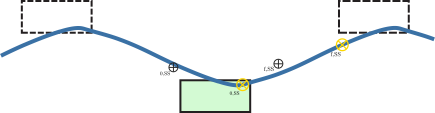
\includegraphics[width=.8\linewidth]{STYLESTUFF/ICPplan3StepComICPrSS.png}
   \caption{Initial (0,SS) and final (f,SS) configurations of \ac{CoM} position (black circle with cross) and \ac{ICP} reference (yellow circle with rotated cross) for \ac{SS} in the $xy$-plane with the parameters from Table \tabref{tab:stepping}. The green area is the current supporting foothold and the blue line is the \ac{ICP} reference trajectory.}
    \label{fig:3foot}
\end{figure}


\begin{figure}[h]
  \begin{subfigure}{0.5\textwidth}
  \centering
  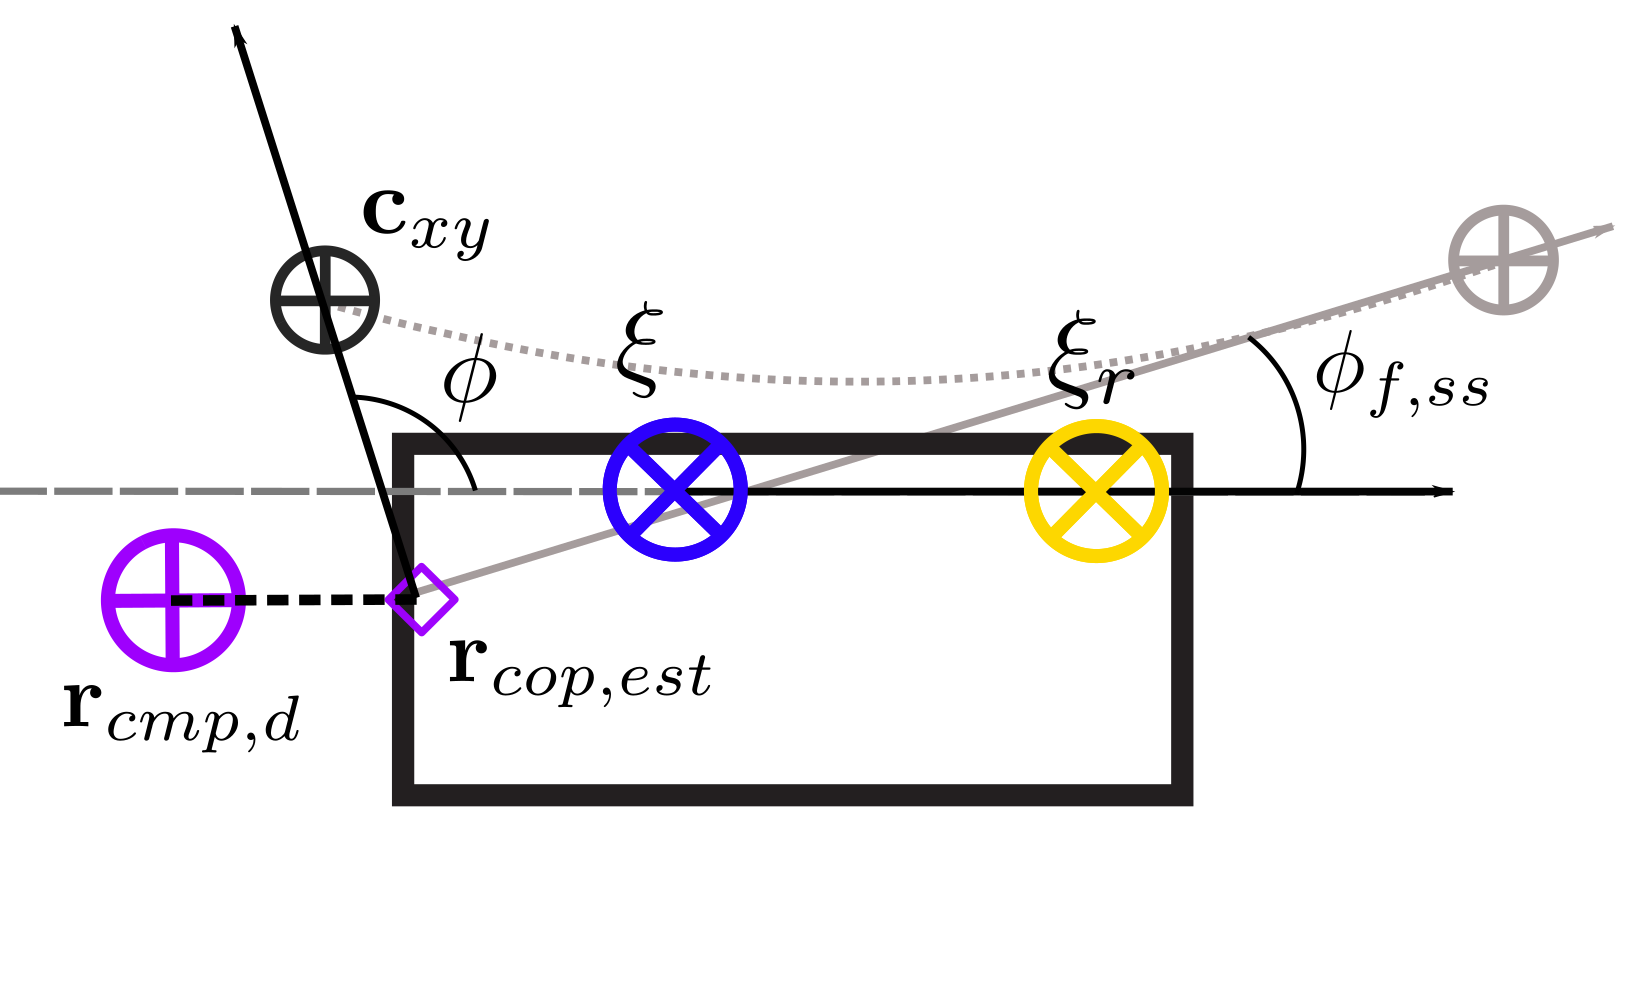
\includegraphics[width=.8\linewidth]{STYLESTUFF/ICPplanStartSSPhiViz.png}
   \caption{}
    \label{fig:phiViza}
  \end{subfigure}
  \begin{subfigure}{0.5\textwidth}
    \centering
  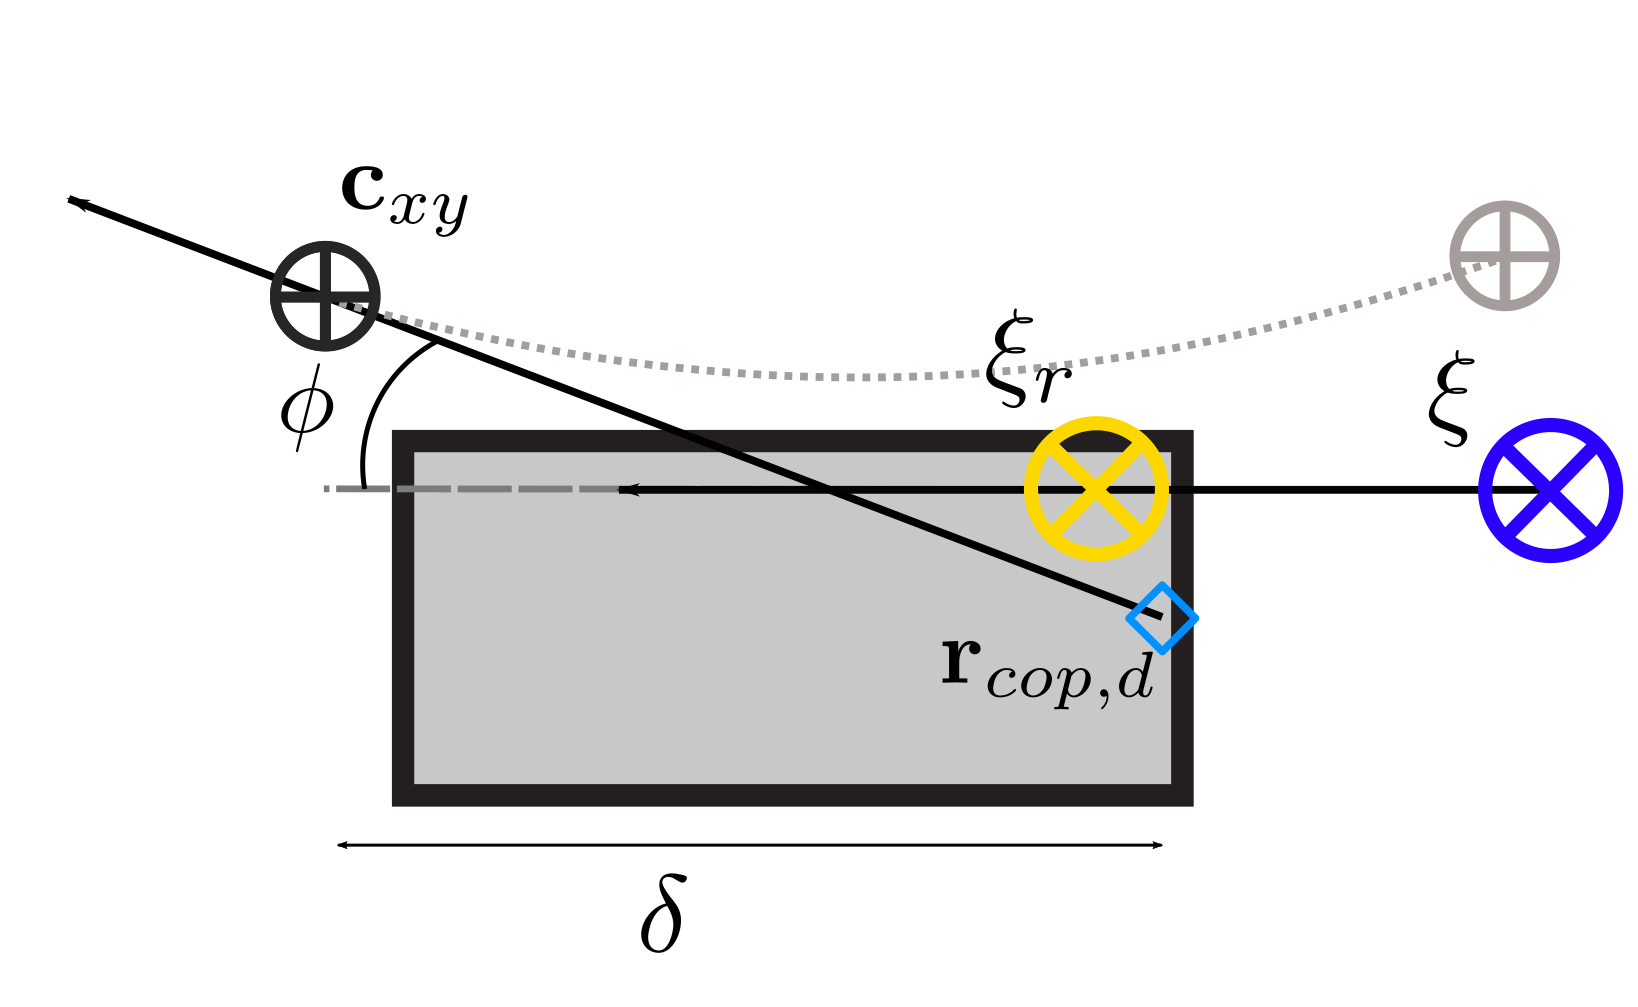
\includegraphics[width=.8\linewidth]{STYLESTUFF/ICPplanStartSSPhiVizNegError.png}
  \caption{}
   \label{fig:phiVizb}
  \end{subfigure}
  \begin{subfigure}{0.5\textwidth}
    \centering
  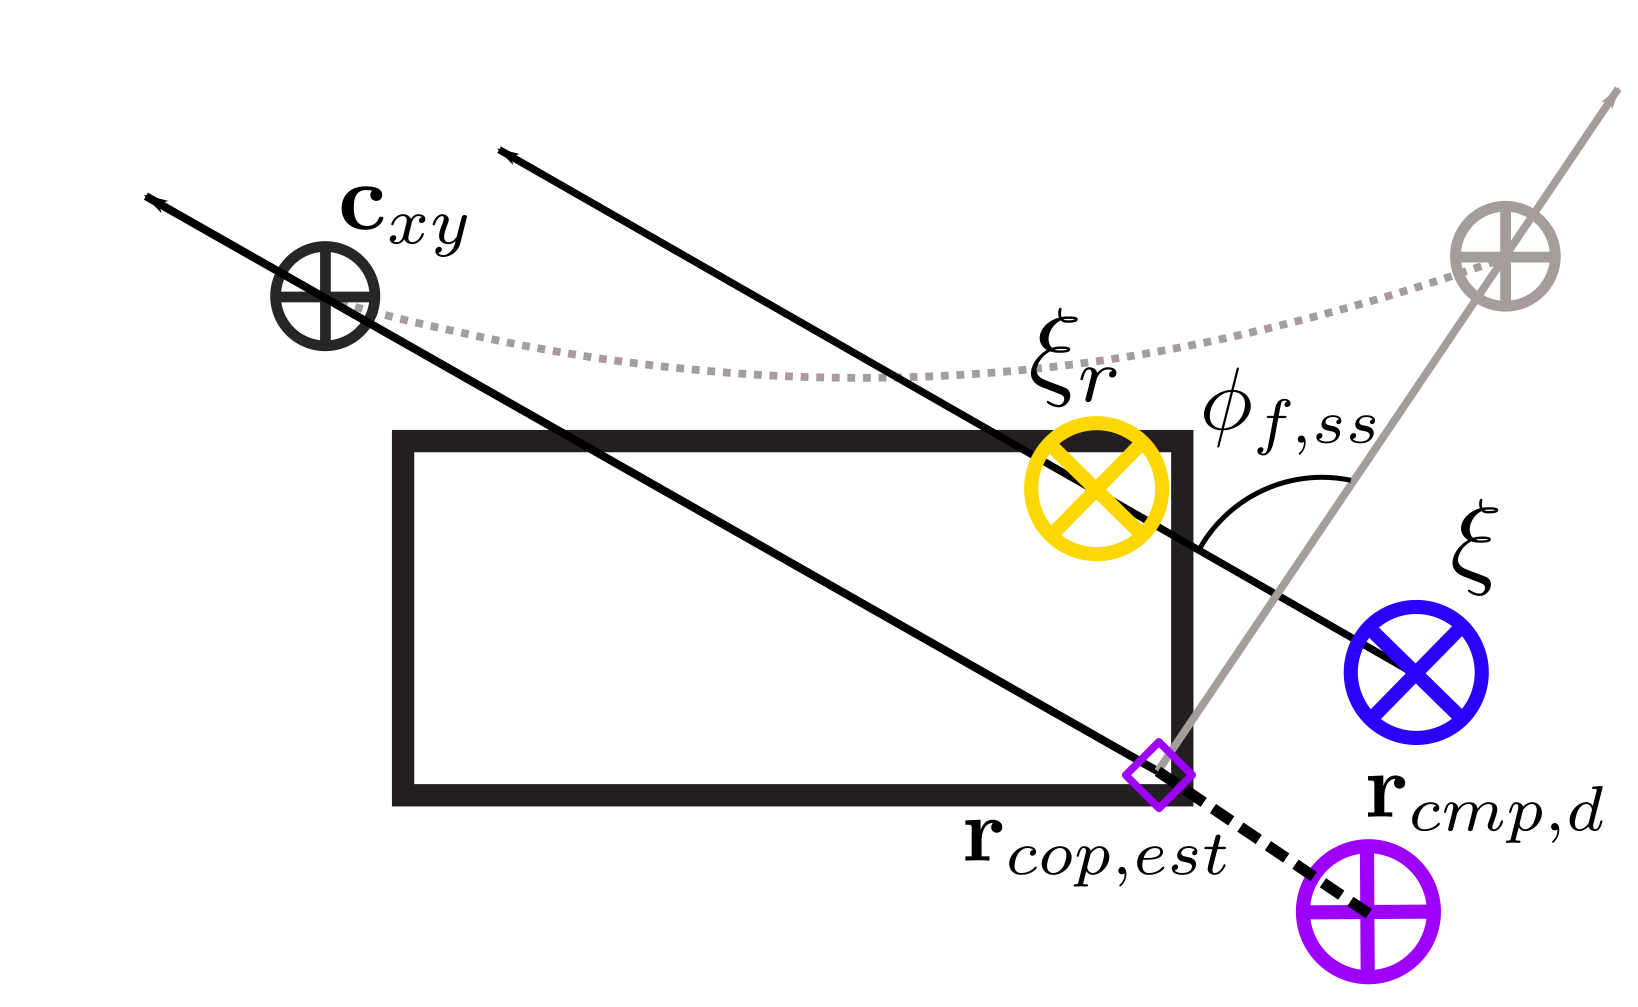
\includegraphics[width=.8\linewidth]{STYLESTUFF/ICPplanStartSSPhiViz0.png}
    \caption{}
     \label{fig:phiVizc}
  \end{subfigure}
  \begin{subfigure}{0.5\textwidth}
    \centering
  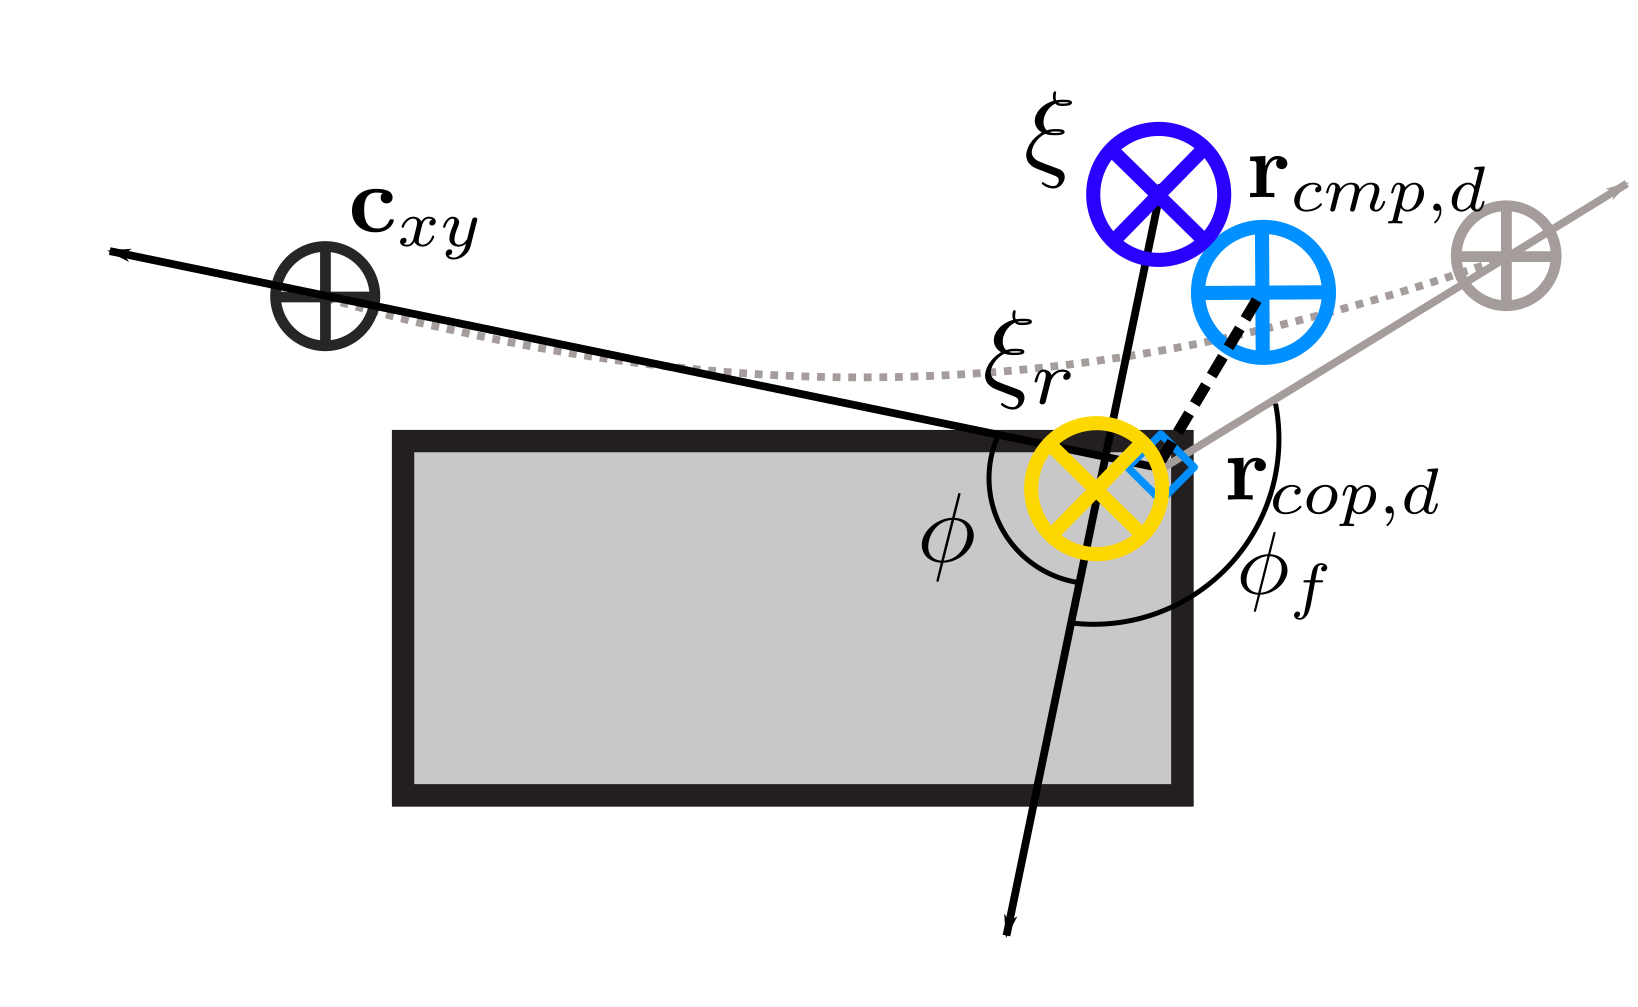
\includegraphics[width=.8\linewidth]{STYLESTUFF/ICPplanStartSSPhiViz90.png}
    \caption{}
     \label{fig:phiVizd}
  \end{subfigure}
    \begin{subfigure}{0.5\textwidth}
    \centering
  \includegraphics[width=.8\linewidth]{STYLESTUFF/ICPplanStartSSPhiVizLeftError.png}
    \caption{}
     \label{fig:phiVize}
  \end{subfigure}
  \begin{subfigure}{0.5\textwidth}
    \centering
  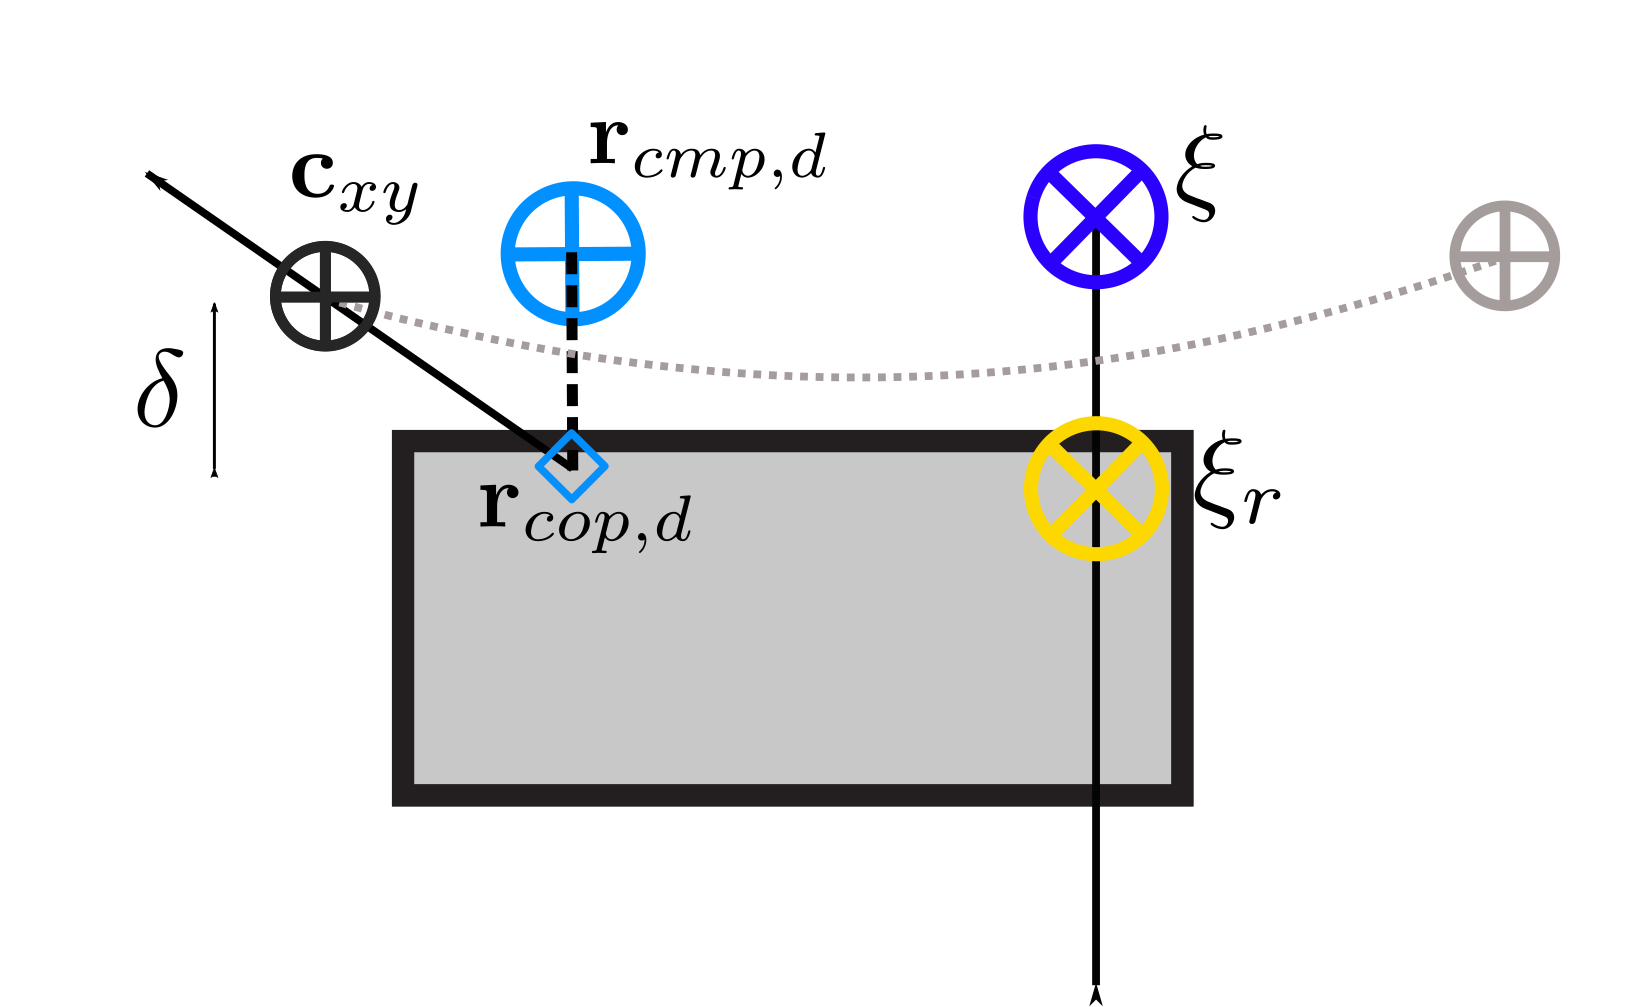
\includegraphics[width=.8\linewidth]{STYLESTUFF/ICPplanStartSSPhiVizRightError.png}
    \caption{}
     \label{fig:phiVizf}
  \end{subfigure}
  \caption{Vizualizations of the error alignment angle for the configuration at start of \ac{SS}, with \ac{ICP} errors: (a) negative in sagital plane, (b) positive in sagital plane, (c) where the error alignment angle is $0$ and (d) where the error alignment angle is orthogonal to the \ac{ICP} error. }
  \label{fig:phiViz}
\end{figure}

%QPbased - Only remarks, not in method?
\subsection{Quadratic Program Based}
One method: use lower weight on vertical momentum rate. To avoid singularity, a feedback based on a virtual spring, priviliged joint accelerations can be projected in the null-space. 

\begin{table}[ht]
\caption{Major affected tasks by $\mathbf{\dot{l}}_{xy,d}$ in whole-body QP, if \ac{CoP} is saturated.} % title of Table
\centering % used for centering table
\begin{tabular}{c c c } % centered columns (4 columns)
\hline\hline %inserts double horizontal lines
Affected Desired & Constraint/Consideration & Centroidal Momentum Rate \\
%heading
\hline % inserts single horizontal line
 $z_d$ & Leg singularity & Linear\\
 $\boldsymbol{\phi}_{body,d}$ & Upper body pose & Angular\\
 $\mathbf{r}_{foot,d}$ &  Touchdown time & Angular\\
%[1ex] % [1ex] adds vertical space
\hline %inserts single line
\end{tabular}
\label{tab:eatqp} % is used to refer this table in the text
\end{table}


% Results
\section{Results}
\subsection{Standing}
Which cases?
\begin{itemize}
	\item Normal limit v.s. height control on normal limit
	\item Normal limit v.s. height control limit -> capture limits
	\item Normal limit high momentum weights v.s. height control on normal limit high momentum weights
\end{itemize}

On what?
\begin{itemize}
	\item joint torques: ankle, knee, hip, back
	\item pose: angular momentum rate, angular momentum, body pose error, CoM
	\item reference points: CMP, CoP, ICP -> Integrated CoP effect and Angular effect > linear momentum
\end{itemize}
\subsubsection{Hardware Tests}
\subsection{Walking}
Focus on strategy.\\
Which cases? 
\begin{itemize}
	\item Normal limit v.s. height control on normal limit
	\item Normal limit v.s. height control limit -> capture limits?
\end{itemize}

On what?
\begin{itemize}
	\item ICP(t) v.s. ICPr(t) v.s. CoP(t) -> compare with assumptions
	\item Swing time and body pose.
\end{itemize}


% Discussion
\section{Discussion}
